\section{Image Classification}
\textbf{Computer Vision} is an interdisciplinary scientific field that deals with how computers can be made to gain \textbf{high-level understanding} from digital images or videos. \\
The connection between Computer Vision and Machine Learning is undergoing a dramatic change: once, most of techniques and algorithms were built upon a mathematical/statistical description of images. Nowadays, machine-learning methods are much more popular: you don't need anymore to go to all these mathematical/statistical models, but you just let a network to resolve a defined task. \\
In case of Classification, the input is an \textbf{image} which corresponds to a set of pixels each associated to a \textit{set of colors}: in each pixel in a colored image you can get three different values (Red, Green, Blue), so we can consider three different images. Videos are sequence of images (frames), so if a frame is $ I \in \mathbb{R}^{R \times C \times 3} $ where 3 represents the RGB values, a video of $T$ frames is defined as
$$
V \in \mathbb{R}^{R \times C \times 3 \times T}
$$
The fourth dimensions is the frame number in the sequence. \\
Dimensions is terribly increasing: a pixel is 1 byte, so without compression a single frame in full HD is stored with $6MB$. Fortunately, visual data are very redundant, thus compressible. A picture is saved in jpeg, which is a lossless compression algorithm that transform the input in a different domain where it can be better compressed. \\

\subsection{Local (Spatial) Transformations}
The simplest operation on an image is a \textit{local transformation} which can be written as $$ G(r,c) = T_U[I(r,c)]
$$
where
\begin{itemize}
    \item I is the input image to be transformed
    \item G is the output
    \item $T_U: \mathbb{R}^3 \rightarrow \mathbb{R}^3$ or  $T_U: \mathbb{R}^3 \rightarrow \mathbb{R}$ is a function
    \item $U$ is neighbourhood, identifies a region of the image that will concur in the output definition
\end{itemize}{}
$T$ operates on $I$ "around" $U$. $T$ can be either linear or nonlinear.\\

\begin{wrapfigure}{r}{5cm}
    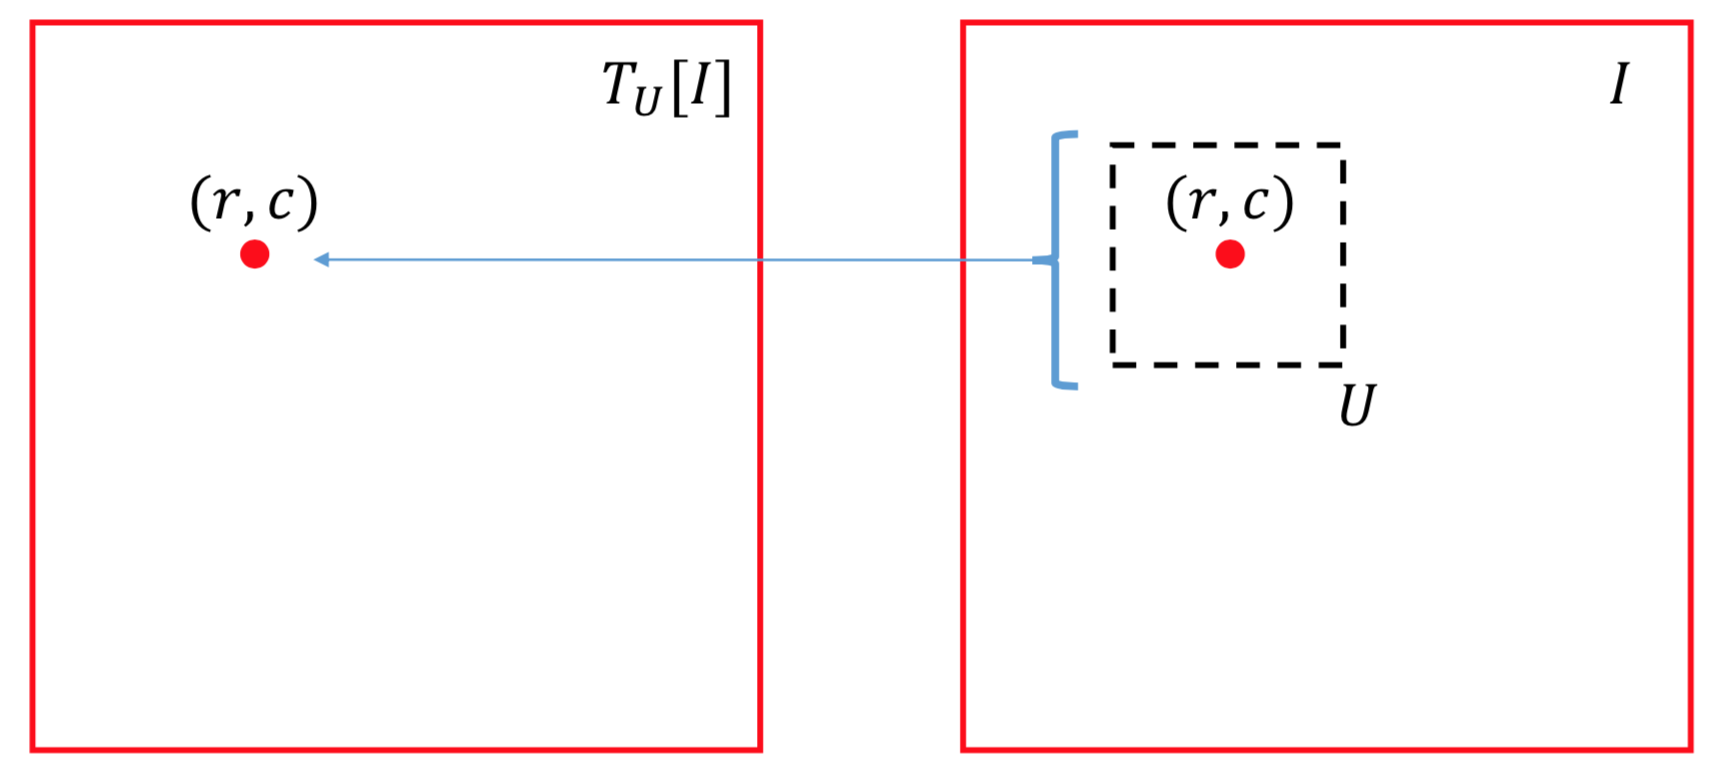
\includegraphics[width=5cm]{images/local_transformation.png}
\end{wrapfigure} 

\textbf{Filter Transformation} takes around each pixel a suitable neighbourhood and defines the output of the transformation by looking only on those values here around.  The output of a filter is a sort of function defined in a neighbour of a pixel. \\
The simplest one is the \textbf{Linear Transformation}: given a pixel, the output of the filter in that pixel is provided by a linear combination of the pixel around that pixel. The output is the linear combination of the weights and the intensity of the values. 
$$ T(I(r,c)) = \sum_{(x, y) \in U} w_i * I(r+x, c+y) = \sum_{(x, y) \in U} w(x, y) * I(r+x, c+y) $$
The parameters of that operation are the weights $w_i$: they can be written like an image, in a matrix. The weights now are arranged in a matrix are called \textbf{Filter $h$}: the filter $h$  entirely defines this operation. This is the Linear Filtering: \\
\begin{minipage}{\linewidth}
        \centering
        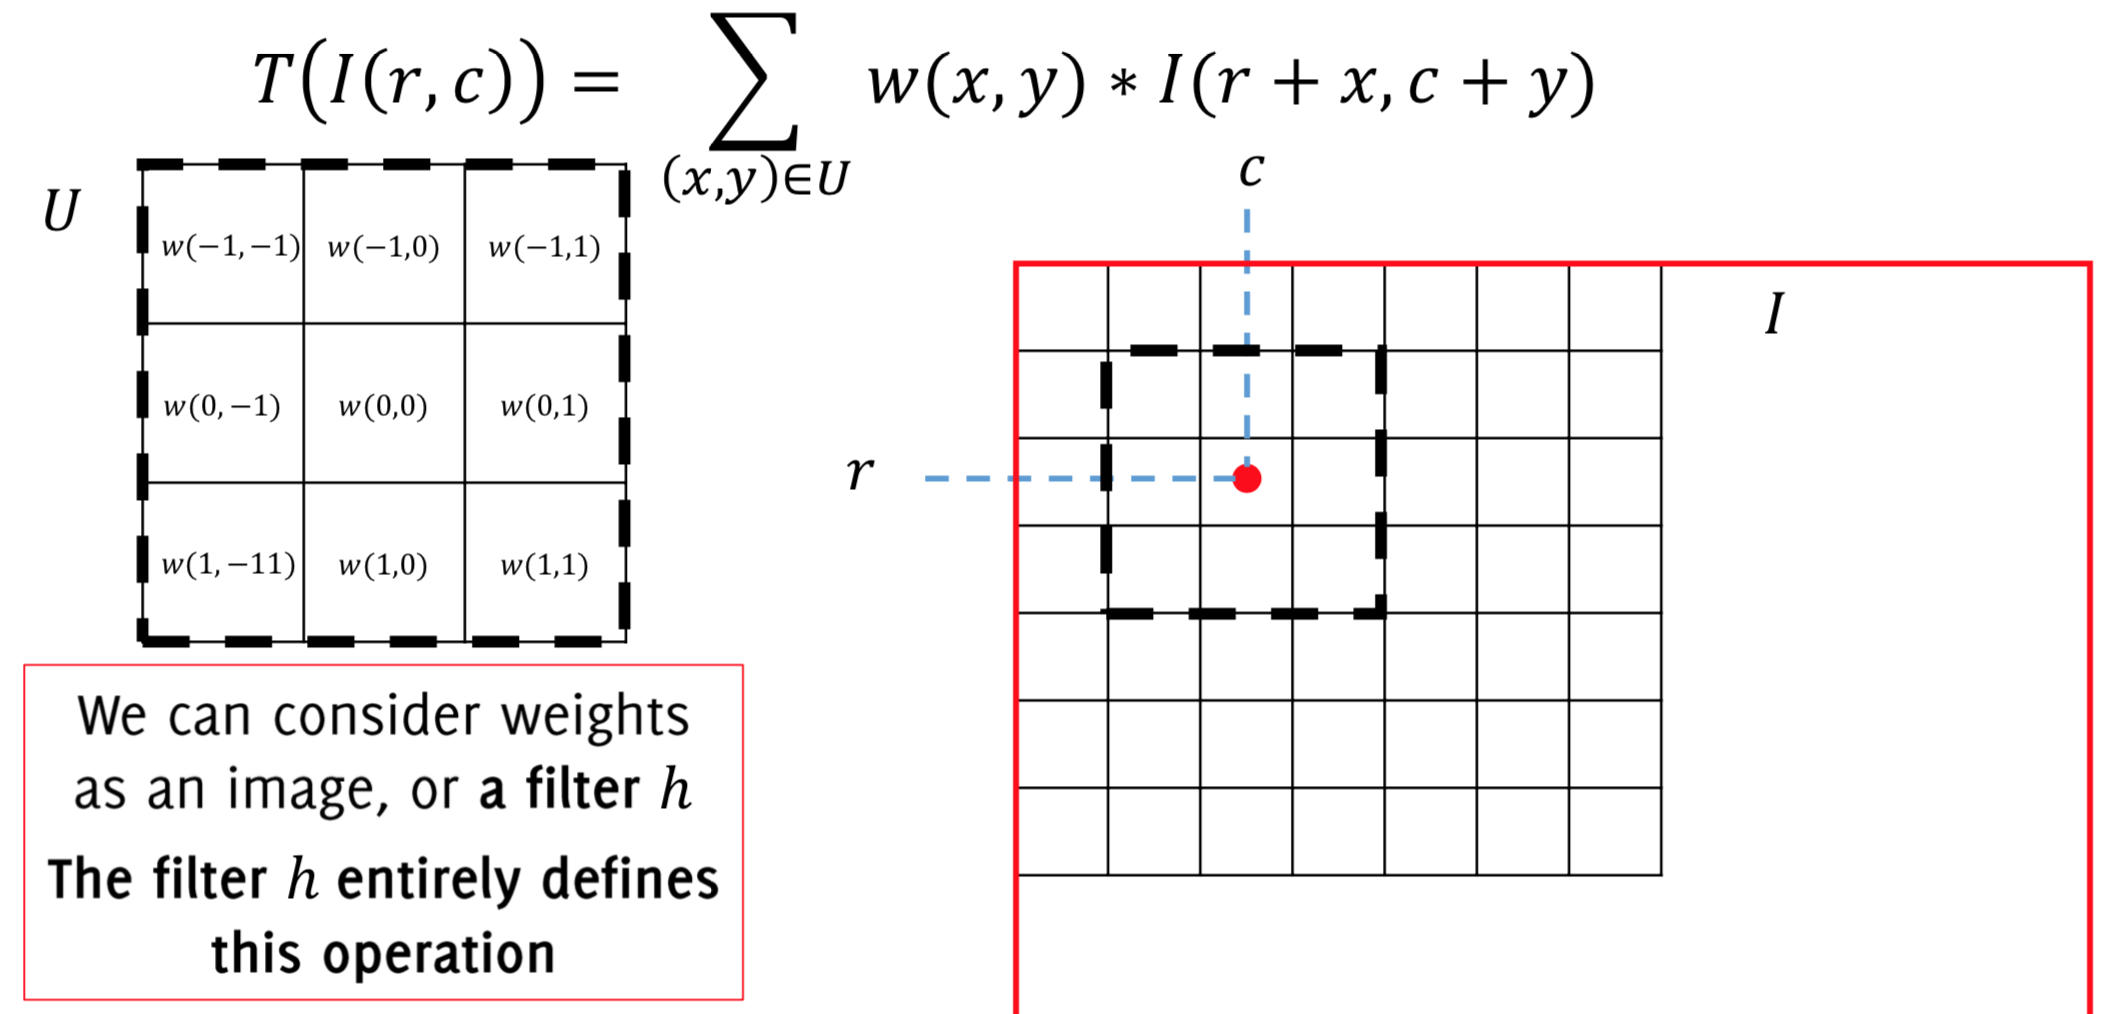
\includegraphics[width=9cm, height=5cm]{images/linear_filter.png}
        %\captionof{figure}{Logical Architecture}
        \label{fig:log_arch}
\end{minipage} \\

The \textbf{Correlation} among a filter $h$ and an image is defined as 
$$
(I \otimes h)=\sum_{u=-L}^{L} \sum_{v=-L}^{L} h(u, v) * I(r+u, c+v)
$$
where the filter $h$ is of size $(2L+1) * (2L+1)$. 
The idea is that you take a filter and 
you overlap it 
%it is like overlapping this filter 
to each location of the image. This operation is performed on each color of the image. \\
"UTK" correlated with "T" example - slide 48: \\
The weights of the filters are 0 or 1 (black or white), when I put the filter over the T in the image, I get the number of pixels equal to 1 in the T. The zeros next to the T is higher, as you move slightly about of the T the intensity of the output increasing since there will be some zeros that will overlap to the T. In this way we can compare images or I can use it to find where the T is in my image. It is enough to know where the T is by taking the local maxima in the correlation output. What you get is where the Ts are. Sometimes we need some sort of normalization to get the things works. 

\subsection{Problem Definitions}
There are different problems to which we focus on:
\begin{itemize}
    \item \textbf{Image Classification}: Assign to an input image $I$ a label $l$ from a fixed set of categories: the classifier gives you the probabilities over each class. $$I \rightarrow l$$
    \item \textbf{Localization}: Assign to an input image $I$ a label $l$ from a fixed set of categories and the coordinates $(x, y, h, w)$ of the bounding box enclosing that object. $$I \rightarrow (x, y, h, w,l)$$
    \item \textbf{Object Detection}: Assign to an input image $I$ \textbf{multiple} labels $\{l_i\}$ from a fixed set of categories, each corresponding to an \textbf{instance of that object}, and the coordinates $\{(x, y, h, w)_i\}$ of the bounding box enclosing \textbf{each} object. 
    $$
    I \rightarrow\left\{(x, y, h, w, l)_{1}, \dots,(x, y, h, w, l)_{N}\right\}
    $$
    \item \textbf{Image Segmentation}: Assign to \textbf{each pixel} of an input image $I$ a label $\{l_i\}$ from a fixed set of categories $\Lambda$ $$ I \rightarrow S(x,y)$$ where $S(x,y) \in \Lambda$. The output of segmentation is an image itself.
    \item \textbf{Instance Segmentation}: Assign to an input image $I$ \textbf{multiple} labels $\{l_i\}$ from a fixed set of categories $\Lambda$, each corresponding to an \textbf{instance of that object}, the coordinates $\{(x, y, h, w)_i\}$ of the \textbf{bounding box enclosing each object}, the \textbf{set of pixels} in each bounding box corresponding to that label 
    $$
    I \rightarrow\left\{(x, y, h, w, l,S)_{1}, \dots,(x, y, h, w, l,S)_{N}\right\}
    $$
    It is like a mix between object detection and segmentation because for each input image you have to assign multiple labels, each one corresponding to instance of an object, to each object you have to provide a bounding box and there is a list of pixel inside the bounding box covered by the object. You can distinguish different persons, in segmentation you cannot.

\end{itemize}
Is this a \textit{challenging problem}? 
\begin{enumerate}
    \item Images are very \textbf{high-dimensional data}.
    \item \textbf{Label Ambiguity}: a label might not uniquely identify the image.
    \item \textbf{Transformation}: you can perform an image transformation that does not change the content, the meaning of the image, but changes the intensity values of the image, so the pixel values.
    \item \textbf{Inter-class Variability}: images belonging to the same class can be dramatically different. 
    \item \textbf{Perceptual Similarity}: it's not pixel-wise similarity, but it means the way you perceive two images to be similar.
\end{enumerate}{}
%We focus on image classification problem. 
%(Esempio su Nearest Neighbourhood Classifier pag.82: you measure the distance between two vector. In case of images you can perform pixel-wise distance among images. \\
%The pixel-wise similarity (the one in the NN-classifier) would not be successful on image. The pixel-wise similarity does not understand the perceptual similarity.) \\

\subsection{Nearest Neighborhood Classifier}
Assign to each test image, the label of the \textbf{closest image} in the training set: 
$$
\hat{y}_{j}=y_{j^{*}}, \quad \text { being } j^{*}=\underset{i=1 \ldots N}{\operatorname{argmin}} d\left(x_{j}, x_{i}\right)
$$
Distances are typically measured as: 
\(d\left(x_{j}, x_{i}\right)=\left\|x_{j}-x_{i}\right\|_{2}=\sqrt{\sum_{k}\left(\left[x_{j}\right]_{k}-\left[x_{i}\right]_{k}\right)^{2}}\)
 
You are measured the distance between two vectors, so basically you are computing a \textit{pixel-wise similarity}. \\
In the same way you can create a K-Nearest Neighborhood Classifier which assigns to each test image, the most frequent label among the \textbf{K-closest} images in the training set. \\
Both the methods will not work since the pixel-wise similarity does not \textit{understand} the perceptual similarity. \\
Pros: 
\begin{itemize}
    \item Easy to understand and implement
    \item It takes no training time
\end{itemize}{}
Cons: 
\begin{itemize}
    \item Computationally demanding at test time
    \item Large training set have to be stored in memory
    \item Rarely practical on images: distances on high-dimensional objects are difficult to interpret
\end{itemize}{}

\subsection{Linear Classifier}
A classifier can be seen as a function that maps an image $x$ to a confidence score for each of the $L$ classes: $$\kappa: \mathbb{R}^d \rightarrow \mathbb{R}^L $$
where $\kappa(x)$ is a $L$-dimensional vector and the i-th component $s_i = [\kappa(x)]_i$. A good classifier associates to the correct class a score that is larger than the scores associated to incorrect classes. \\
Dealing with images, the input \textbf{x} belongs to $\mathbb{R}^d$ where $d$ is the dimension of the image. The Linear Classifier get an input image and extract a set of scores for each class, but need to be linear. In Linear Classification, $\kappa$ is a \textbf{linear function}: 
$$ \kappa(x) = Wx + b $$
where $W \in \mathbb{R}^{L \times d}$ are the weights , $b \in \mathbb{R}^L$ is the bias, both are the parameters of the classifier. \\ 

\begin{minipage}{\linewidth}
        \centering
        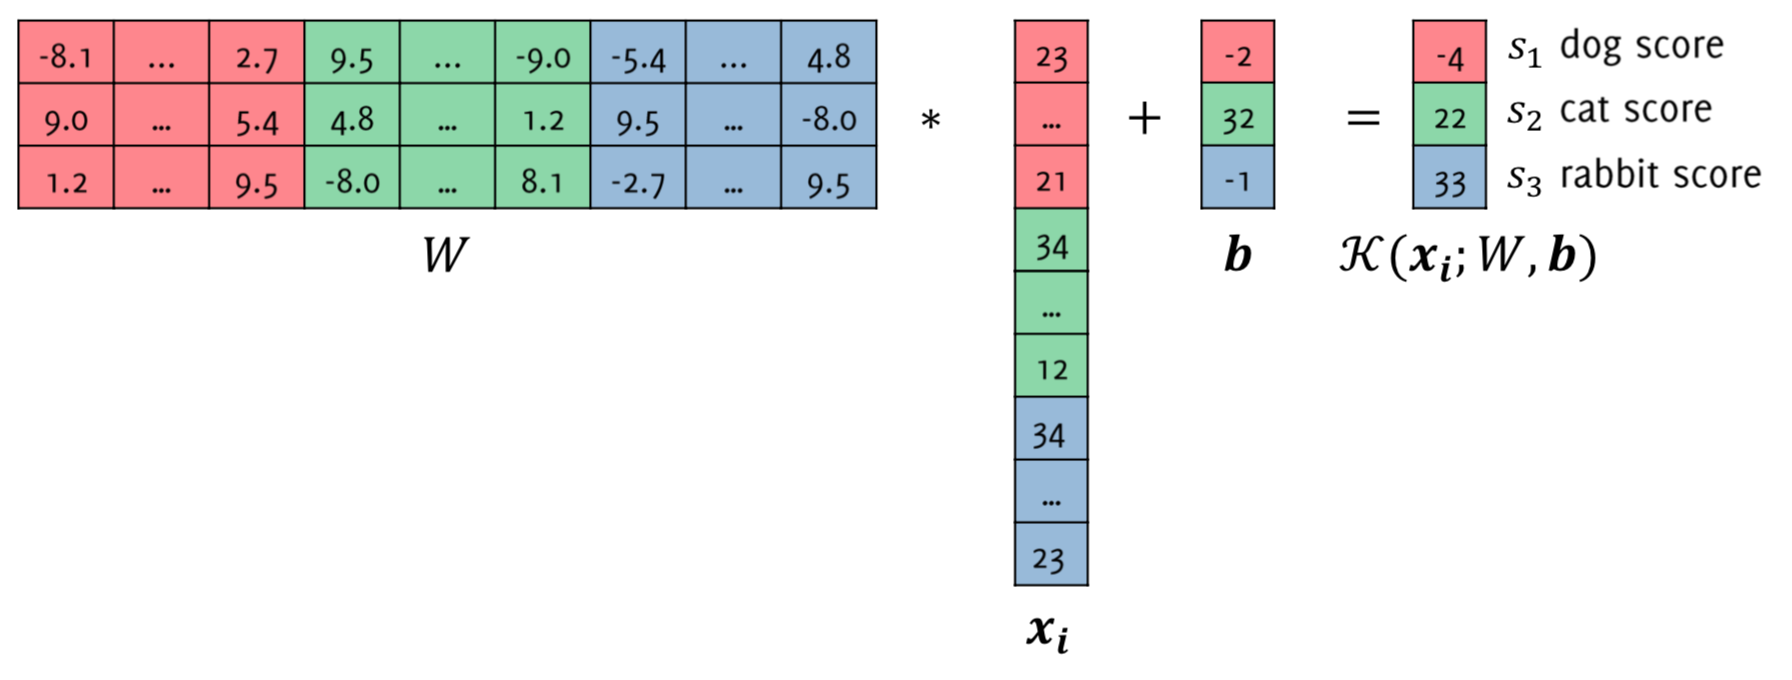
\includegraphics[width=12cm, height=5cm]{images/linear_class.png}
\end{minipage}

So you need to perform a linear transformation of the input vector and what you obtain as output is a vector in which each component is the score assigned to each class. In the \textit{weights matrix}, each row corresponds to the weights related to a class; a row has the same size $d$ of the input image vector $x_i$. To create the input image vector, starting from an image (and from the red image of an RGB), you unroll it column-wise: from top-left corner, you read column wise and move from red to green to blue images. 
%and you start all the red pixel in the top part of your vector, then you move to the green and at the end to the blue part. 
This corresponds to your vector $x_i$, your input image i. So the linear classifier operation is row (a class) times column (your input), which output is a vector of L values, one for each class. Adding the bias we get the last output of the classifier as results. The classifier assign to an input image the class corresponding to the largest score 
$$
\hat{y}_{j}=\underset{i=1, \ldots, L}{\operatorname{argmax}}\left[s_{j}\right]_{i}
$$
The parameters of this classifier are the weights, so we need to train this classifier in order to learn the weights: weights indicate which are the most important pixels / colors. Also the value of bias is in your parameters. The number of parameters are $d \times L + L$, which are the exactly number of parameter in a layer of a neural network. \\
Given a training set and a loss function, define the parameters that minimize the loss function over the whole training set, so in case of linear classifier: 
$$
[W, b]=\operatorname{argmin}_{W \in \mathbb{R}^{L \times d}, b \in \mathbb{R}^{L}} \sum_{\left(x_{i}, y_{i}\right) \in T R} \mathcal{L}\left(\boldsymbol{x}, y_{i}\right)+\lambda \mathcal{R}(W, b)
$$
The loss function has to be regularized to achieve a unique solution satisfying some desired property, where $\lambda > 0$ is a parameter balancing the two terms. \\ 
\subsubsection{Geometric Interpretation of a Linear Classifier}
Given a classifier already trained with $W$ and $b$. The first intuition, if you take the matrix $W$ and input $x$, you can add the bias and compute the scores. What contribute to the scores of the first class is just the first row of the matrix. So you can see the i-th row of $W$ as the classifier corresponding to the i-th class. It just a matter of computing a inner product between $w_i$ and an input $x$.\\
%(pag 106)
If we were in two-dimension, an image is like a point, each row of the matrix identifies that linear function which corresponds to a set of (hyper-)plane where if the input point is above or below that plane it means that the point belongs or not to a class. So what you are doing is looking at your image in a $d$-dimensional space and trying to separate classes by hyper-plane and dividing your input images by 'putting' them in one of these hyper-planes. \\ \\
\textit{Geometric interpretation}: you take an high-dimensional space, try to separate images through hyper-planes and you define the hyper-plane in order to do the best you can do for the given training set. \\

Another interpretation: taking $W$, a row of $W$ contains $d$ values which is the same size as image, so we can reshape it to generate an image and visualize it like an image $\rightarrow$  Template. So you multiply this template for your input and sum the bias for each template and this is exactly correlation that we have seen before. The Linear Classifier is just learning some template to which it performs correlation against and you provide as output the class of the template that provides you the largest response. 